\documentclass[12pt,a4paper]{ctexart}
\usepackage{ulem}
\usepackage{circuitikz}
    \def\V{\ \mathrm{V}}
    \def\mV{\ \mathrm{mV}}
    \def\kV{\ \mathrm{KV}}
    \def\KV{\ \mathrm{KV}}
    \def\MV{\ \mathrm{MV}}
    \def\A{\ \mathrm{A}}
    \def\mA{\ \mathrm{mA}}
    \def\kA{\ \mathrm{KA}}
    \def\KA{\ \mathrm{KA}}
    \def\MA{\ \mathrm{MA}}
    \def\O{\ \Omega}
    \def\mO{\ \Omega}
    \def\kO{\ \mathrm{K}\Omega}
    \def\KO{\ \mathrm{K}\Omega}
    \def\MO{\ \mathrm{M}\Omega}
    \def\Hz{\ \mathrm{Hz}}
    \def\N{\mathbb{N}}
    \def\F{\mathbb{F}}
    \def\Z{\mathbb{Z}}
    \def\Q{\mathbb{Q}}
    \def\R{\mathbb{R}}
    \def\C{\mathbb{C}}
    \def\T{\mathbb{T}}
    \def\S{\mathbb{S}}
    %\def\A{\mathbb{A}}
    \def\I{\mathscr{I}}
    \def\d{\mathrm{d}}
    \def\p{\partial}
    \usepackage[UTF8]{ctex}
    \usepackage{hyperref}
    \hypersetup{
        colorlinks=true,
        citecolor={blue},
        linkcolor={blue},
        urlcolor={orange},
    }
    \usepackage{amsmath}
    \usepackage{mathrsfs}
    \usepackage{amssymb}
    \usepackage{pifont}
    \usepackage{extarrows}
    \usepackage{multicol}
    \usepackage[a4paper]{geometry}
        \geometry{top=0.75in}
        \geometry{bottom=0.75in}
        \geometry{left=0.75in}
        \geometry{right=0.75in}
        \geometry{marginparwidth=1.75cm}
    \usepackage{amsthm}
        \newtheoremstyle{MyLineTheoremStyle}
            {11pt}
            {11pt}
            {\kaishu}
            {}
            {\bfseries}
            {:\ \ }
            {.5em}
            {\textbf{#1}\thmnumber{#2}\ \ (\,\textbf{#3}\,)}
        \theoremstyle{MyLineTheoremStyle}
        \newtheorem{LineTheorem}{Theorem.\,}
        \newtheoremstyle{MyBlockTheoremStyle}
            {11pt}
            {11pt}
            {\kaishu}
            {}
            {\bfseries}
            {:\\ \indent}
            {.5em}
            {\textbf{#1}\thmnumber{#2}\ \ (\,\textbf{#3}\,)}
        \theoremstyle{MyBlockTheoremStyle}
        \newtheorem{BlockTheorem}[LineTheorem]{Theorem.\,}
        \newtheoremstyle{MySubsubsectionStyle}
            {11pt}
            {11pt}
            {}
            {}
            {\bfseries}
            {\\ \indent}
            {0pt}
            {\textbf{#3}}
        \theoremstyle{MySubsubsectionStyle}
        \newtheorem{definition}{}
    \usepackage{xcolor}
    \usepackage[strict]{changepage}
    \usepackage{framed}
        \definecolor{graybox_color}{rgb}{0.95,0.95,0.96}
        \newenvironment{graybox}{
        \def\FrameCommand{
        \hspace{1pt}
        {\color{gray}\small \vrule width 2pt}
        {\color{graybox_color}\vrule width 4pt}
        \colorbox{graybox_color}
        }
        \MakeFramed{\advance\hsize-\width\FrameRestore}
        \noindent\hspace{-4.55pt}
        \begin{adjustwidth}{}{7pt}
        \vspace{2pt}\vspace{2pt}
        }
        {
        \vspace{2pt}\end{adjustwidth}\endMakeFramed
        }

    \usepackage{matlab-prettifier}
        \lstset{style=Matlab-editor}
    \usepackage[most]{tcolorbox}
    \usepackage{listings}
        \tcbuselibrary{listings, skins, breakable}
        \newfontfamily\codefont{Consolas}
        \lstdefinestyle{MatlabStyle_inc}{
            language=Matlab,
            basicstyle=\small\ttfamily\codefont,
            breakatwhitespace=false,
            breaklines=true,
            captionpos=b,
            keepspaces=true,
            numbers=left,
            numbersep=15pt,
            showspaces=false,
            showstringspaces=false,
            showtabs=false,
            tabsize=2,
            xleftmargin=15pt,
            %frame=single,
            frame=shadowbox,
            %frameround=tttt,
            framextopmargin=0pt,
            framexbottommargin=0pt,
            framexleftmargin=5pt,
            framexrightmargin=5pt,
            rulesepcolor=\color{red!20!green!20!blue!20},
        }
        \lstdefinestyle{MatlabStyle_src}{
            language=Matlab,
            basicstyle=\small\ttfamily\codefont,
            breakatwhitespace=false,
            breaklines=true,
            captionpos=b,
            keepspaces=true,
            numbers=left,
            numbersep=15pt,
            showspaces=false,
            showstringspaces=false,
            showtabs=false,
            tabsize=2,
        }
        \newtcblisting{matlablisting}{
            top=0pt,
            bottom=0pt,
            left=-5pt,
            right=-5pt,
            listing only,
            listing style=MatlabStyle_src,
            breakable,
            colback=white,
            colframe=black!0,
        }
        \lstset{
            style=MatlabStyle_inc,
        }

    \usepackage{booktabs}
    \usepackage{tabularray}
    \usepackage{longtable}
    \usepackage{diagbox}
    \usepackage{graphicx}
    \usepackage{svg}
        \svgsetup{
            inkscapeexe = C:/aa_MySame/inkscape/bin/inkscape.exe,
            inkscapelatex = false                 
        }
    \usepackage{subcaption}

    \usepackage{caption}
        \captionsetup[figure]{name=图}  
        \captionsetup[table]{name=表}
        \captionsetup{
            labelfont=bf,
            textfont=bf,
            font=small  
        }
    \usepackage{float}

    \newcommand*\circled[1]{\tikz[baseline=(char.base)]{\node[shape=circle,draw,inner sep=0.8pt, line width = 0.03em] (char) {\small \bfseries #1};}}

    \usepackage{enumitem}
        \setlist[enumerate]{
            label=(\arabic*),
            ref=\arabic*,
            itemsep=0pt, parsep=0pt, topsep=0pt, partopsep=0pt, leftmargin=3.5em} 
        \setlist[itemize]{itemsep=0pt, parsep=0pt, topsep=0pt, partopsep=0pt, leftmargin=3.5em}
        \newlist{circledenum}{enumerate}{1}
        \setlist[circledenum,1]{  
            label=\protect\circled{\arabic*},
            ref=\arabic*,
            itemsep=0pt, parsep=0pt, topsep=0pt, partopsep=0pt, leftmargin=3.5em
        }  

        \renewcommand\thefootnote{\ding{\numexpr171+\value{footnote}}}
        \bibliographystyle{unsrt}
        \newcommand{\upcite}[1]{\textsuperscript{\cite{#1}}}
        \newcommand{\cnabstractname}{序言}
        \newenvironment{cnabstract}{
            \par\Large
            \noindent\mbox{}\hfill{\bfseries \cnabstractname}\hfill\mbox{}\par
            \vskip 2.5ex
            }{\par\vskip 2.5ex}

    \usepackage{fontspec}
        \setmainfont{SimSun}
        \setCJKmainfont[AutoFakeBold=3]{SimSun}
        \setmainfont{Times New Roman}

\usepackage{titlesec,graphicx,amsmath,amssymb,tikz}
\usetikzlibrary{shapes.geometric,arrows}
\tikzstyle{startstop}=[rectangle,rounded corners,minimum width=1cm,minimum height=0.5cm,text centered,draw=black,fill=red!30]
\tikzstyle{process}=[rectangle,minimum width=1cm,minimum height=0.5cm,text centered,draw=black,fill=orange!30]
\tikzstyle{arrow}=[thick,->,>=stealth]
\graphicspath{{img/}}
\titleformat{\section}{\normalfont\large\bfseries}{\thesection}{1em}{}
\title{
    {\Large Research Process Summary}\\
    {\large The Relationship Between Internet Meme Culture and Cyberbullying}
}
\author{
    {\small Team Members: Li Weicilin, Pan Hanlin, Zhang Shuo, Zhang Shukai}\\
}
\date{Last Updated: June 6, 2025}

\begin{document}
\maketitle
\tableofcontents
\newpage

\section{Research Introduction}
\subsection{Background}

Keywords: Meme culture, Cyberbullying.

Abstract culture has undergone a process of dissemination, starting from live streaming rooms, spreading to social media, and eventually permeating the entire online space. This study examines the dynamic interplay between Abstract Culture and Cyberbullying within today's digital ecosystem.

Abstract Culture originated from unconventional behaviors and rhetoric deliberately employed by live streamers to attract viewership. Its dissemination was propelled by anti-fans, who propagate livestream conflicts by launching systematic smear campaigns on social media platforms like Weibo. These attacks reframed targets as "villains" or "reactionaries," constituting a novel form of cyberbullying centered on public stigmatization.

To evade content moderation, anti-fans developed Abstract Language—a linguistic tool leveraging semantic ambiguity, metaphorical abbreviations, and polysemic symbols. This enabled covert propagation of hostile content.

As Abstract Language permeated mainstream internet culture, its function underwent fundamental transformation: ordinary users detached it from its original malicious intent, repurposing it as social entertainment symbols. Case studies (e.g., violent memes like "牢大" and "耄耋(猫爹)") reveal how widespread adoption dissociated such expressions from aggression, recasting them as neutral humor. Collective reinterpretation where users derive divergent meanings from identical phrases generated communal amusement, facilitating Abstract Culture's deep integration into daily online communication and reshaping digital cultural norms.

\subsection{Research Significance}

This  study  holds  significant value by  illuminating the  complex  inter- play between Abstract Culture and cyberbullying in the digital ecosystem.

The research reveals a pro- found cultural transformation: as Abstract Language permeated mainstream online spaces, ordinary users divorced it from its original malicious intent. Case studies demonstrate how widespread adoption reinterpreted these ex- pressions as neutral social entertainment symbols. This collective reappropri- ation—where users derive divergent, often humorous meanings from identical phrases—effectively dissolved their aggressive connotations.This insight fundamentally advances our understanding of semiotic fluidity in internet culture.As an increasingly popular form of communication in the Internet age, it is of great significance to explore the dynamic role of abstract culture on online language in order to limit the emerging cyberbullying problem that may exist in the Internet age

\subsection{Research Questions}

Given the general background of internet meme culture development and the definition, nature, and impact of cyberbullying, our research team aims to investigate the evolving relationship between meme culture and cyberbullying, as well as its influence on a broad online population. This issue is divided into three key aspects:

Temporal Framework of Internet Meme Culture: Due to the rapid and diversified development of internet meme culture, establishing an up-to-date information framework is essential. This includes analyzing its role in online communication, practical utility, and circulation (i.e., widespread adoption among netizens). A clear understanding of this aspect will facilitate further analysis of meme culture.

Origins of Cyberbullying in Online Communication: We seek to examine how violent language emerges on internet platforms, particularly in exchanges involving abstract online language. This will allow us to analyze instances of cyberbullying that arise within meme-based communication.

Dissipation of Cyberbullying Through Abstraction: Over time, cyberbullying behaviors may spread beyond perpetrator circles, with violent language being abstracted, popularized, and eventually neutralized through humor or widespread use. Our team will also analyze this process of dissipation.

\subsection{Hypotheses}

The inherent connections within meme content facilitate rapid dissemination through familiarity.

As abstract vocabulary gains popularity, its violent connotations diminish while cultural influence persists.

All meme content undergoes similar cycles of generation and transformation.

Most cyberbullying stems from conflicts between anonymous groups and identifiable individuals/groups, where anonymity enables both meme-based attacks and evasion of platform oversight.

\subsection{Research Objectives}

This study adopts a mixed-methods approach combining survey research and computational analysis to examine the relationship between internet meme culture and cyberbullying.

The survey component involves administering a structured questionnaire to assess participants' familiarity with meme culture and experiences with cyberbullying. The questionnaire collects demographic data and evaluates meme comprehension through semi-open questions, while also measuring cyberbullying exposure through scenario-based items. This design captures subjective perceptions across diverse online communities.

For digital behavioral analysis, we employ web scraping to track violent meme evolution on platforms like Bilibili. The automated data collection focuses on comment sections, followed by NLP processing to quantify meme usage patterns and contextual shifts. Analytical techniques include frequency distribution mapping, sentiment analysis, and network visualization to examine how aggressive language transforms through meme circulation.

The integrated analysis correlates survey responses with observed behavioral patterns, using statistical models to test relationships between meme adoption and the normalization of formerly hostile expressions. Methodological rigor is ensured through pilot testing, reliability checks, and validation procedures across both research components.

This dual-method design enables comprehensive investigation of both conscious perceptions and unconscious behavioral manifestations within meme-mediated online interactions.

\begin{figure}[htbp]
    \centering
    \resizebox{\textwidth}{!}{
        \begin{tikzpicture}[node distance=2cm]
            \node (start)[startstop]{Meme Culture \& Cyberbullying};
            \node (process1)[process,below of=start,yshift=0cm,xshift=-4cm]{Meme Culture Definition/Properties};
            \node (process2)[process,below of=start,yshift=0cm,xshift=4cm]{Cyberbullying Definition/Characteristics};
            \node (process3)[process,below of=start,yshift=-2cm,xshift=0cm]{Interrelationship Analysis};
            \node (process4)[process,below of=process3,yshift=0cm,xshift=-3cm]{Cyberbullying Emergence};
            \node (process5)[process,below of=process3,yshift=0cm,xshift=3cm]{Violence Neutralization};
            \node (end)[startstop,below of=process3,yshift=-2cm,xshift=0cm]{Analytical Results};
            \draw [arrow] (start) -- (process1);
            \draw [arrow] (start) -- (process2);
            \draw [arrow] (process1) -- (process3);
            \draw [arrow] (process2) -- (process3);
            \draw [arrow] (process3) -- (process4);
            \draw [arrow] (process3) -- (process5);
            \draw [arrow] (process3) -- (end);
            \draw [arrow] (process4) -- (end);
            \draw [arrow] (process5) -- (end);
        \end{tikzpicture}
    }
    \caption{Research Framework}
    \label{fig:research_process}
\end{figure}
\newpage

\section{Research Methods}

\subsection{Crawlerweb}

In order to explore the influence of abstract culture on the characteristics of online language, we designed and constructed a public opinion evaluation system based on dictionaries and Jieba word segmentation tools in order to explore the attention to original issues, the aggressiveness of comments and the spread of Internet memes in public comments. The system starts from three aspects: topic relevance evaluation, aggression evaluation and meme association evaluation, and provides visual and quantitative analysis support for the overall content characteristics of the comment area by constructing multi-level dictionaries and frequency-based quantitative methods.

Data acquisition:

Python-based video comment area information collection: automatic crawling of comments on videos specified by bilibili and their multi-level replies. The program first simulates normal user access by setting the browser request header to avoid being intercepted by the anti-crawler mechanism. The main function requests the comment API of Bilibili by pagination, obtains all first-level comments, and recursively captures all second-level and lower-level replies under each comment to ensure the integrity of the comment data. Each comment and reply extracts key information such as the user's nickname, comment content, the user replied to, the comment level, gender, rating, number of likes, and reply time. All acquired review data is eventually saved as a CSV file for further analysis.

\begin{figure}[htbp]
    \centering
    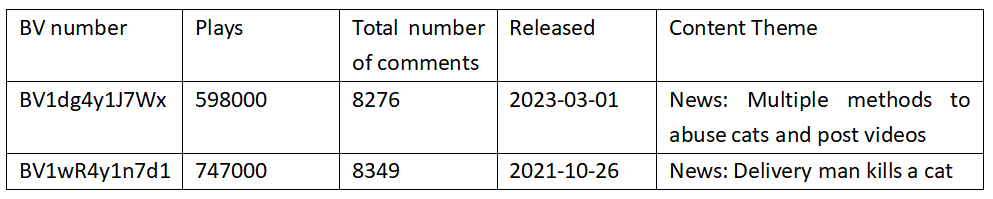
\includegraphics[width=0.8\textwidth]{img/data_sources_1.png}
    \caption{Overview of data sources}
    \label{fig:data_sources_1}
\end{figure}
\newpage

For the data used for dictionary construction, we used the comment areas of CCTV Video and Sichuan Observation on the two news reports, which better covered the topics of "流浪猫问题" and "虐猫行为" born from the meme of “耄耋”, and at the same time had sufficient number of comments, which is beneficial for accurately obtaining the dictionary content.

\begin{figure}[htbp]
    \centering
    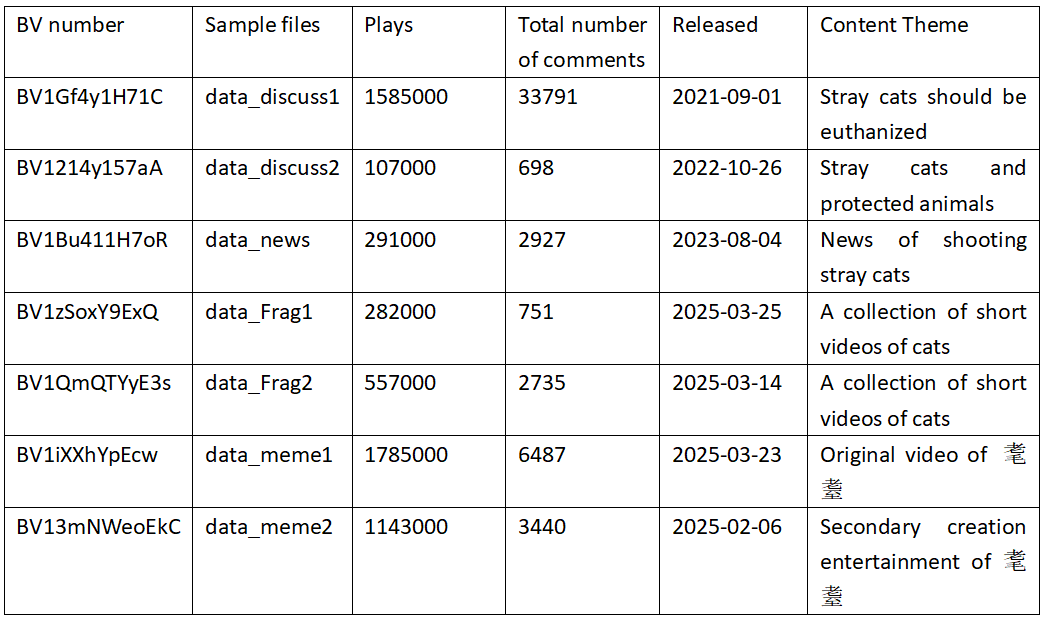
\includegraphics[width=0.8\textwidth]{img/data_sources_2.png}
    \caption{Overview of data sources}
    \label{fig:data_sources_2}
\end{figure}
\newpage

According to a number of video samples on different topics obtained by manual screening of video content, the BV1Gf4y1H71C video is a discussion on how to deal with the problem of stray cats, and the author believes that euthanasia needs to be used to solve the flood of stray cat population; The authors of BV1214y157aA use radical language to express a critique of stray cats as an invasive species that threaten the ecology; BV1Bu411H7oR is a news story about someone using a bow to shoot stray cats in a neighborhood; BV1zSoxY9ExQ and BV1QmQTYyE3s are a collection of short videos about cat behavior; BV1iXXhYpEcw documents a feral cat breaking into a home and displaying extreme aggression, which is now widely referred to as "耄耋" in abstract culture. BV13mNWeoEkC is a ghost animal entertainment video created using the video data of "耄耋".

Evaluation system construction:

Since the content of the three evaluation systems is natural language text, the intuitive evaluation method is to statistically evaluate the specific text content. Therefore, research first needs to establish a dictionary.

In order to fully and objectively define the main direction and topic of the discussion of the occurrence scene of the "耄耋" stalk and the stray cat problem, this study first collected the data of two news videos about the stray cat problem in the comment area, and obtained a topic relevance dictionary content that comprehensively reflects the details of the discussion of the stray cat problem by counting the high-frequency words in the comment area and manually screening the stray cat problem.

Jieba: An efficient and easy-to-use Chinese word segmentation tool that can accurately divide continuous Chinese text into words, supports three word segmentation modes: exact mode, full mode and search engine mode, and allows users to optimize the word segmentation effect in specific fields through custom dictionaries. It also provides keyword extraction and part-of-speech annotation functions, which are widely used in text analysis, information retrieval and natural language processing tasks, and is one of the basic tools for processing Chinese text.

Combined with the language sentiment color analysis of jieba, we screened the above high-frequency words for the second time, and obtained high-frequency words with more obvious negative emotions, which obviously not only have strong aggression, but also have a stronger correlation with the discussion of stray cats, so as to obtain a more accurate judgment of the offensive dictionary content of aggression in the comment area.

LDA: A classic unsupervised machine learning algorithm used primarily for topic modeling of text data. It analyzes the distribution of words in a document, automatically identifies the underlying topic structure, and represents each document as a probability mix of multiple topics, while each topic is represented as a probability distribution of a series of related words.

Meme association evaluation based on preset dictionaries: The program automatically identifies the "comment content" and "like" fields in each file, and determines whether each comment contains the specified primary or secondary meme keyword. If the primary keyword appears in the comment, the score will be accumulated according to the number of likes (1 if the number of likes is 0), and the score will be increased by 1 if the secondary keyword appears. Each comment that contains any of the prompt keywords counts towards the "Prompt Comments". Finally, the program counts the total number of valid comments, the number of meme comments and the normalized meme influence score (total score/number of comments) of each file, and displays the meme influence of each file in the form of a histogram, and outputs detailed statistical results on the terminal, which is convenient for detailed comparison of the propagation and influence of memes in different data sources.

Topic relevance evaluation based on preset dictionaries: The program realizes the analysis of the native context shift of "memes" on multiple CSV comment data files. The program automatically recognizes the content of the comments in each file, tokenizes each comment, and assigns different points (4, 2, and 1 points) to each word according to a custom hierarchical dictionary (primary, secondary, tertiary). After the scores of each comment are accumulated, the average native index of each file is calculated, and the distribution of the native index of each file is displayed in the form of a bar chart. The program will also output the total number of comments and the average native index of each file in the terminal, which is convenient for intuitive comparison and analysis of the originality and offset degree of the "meme" context in different data sources.

In order to investigate the characteristics of the discussion content in the comment area, we combined jieba and LDA to implement a Chinese text topic analysis system: through LDA topic modeling, the core topics and keyword distribution of the comment content of each document were extracted. The system first preprocessed the original text such as Chinese word segmentation and stop word filtering, and then constructed a word frequency matrix and trained an LDA model to identify the five main topics and their representative keywords in each file. Topic diversity is quantified by calculating the normalized entropy value, and finally the visualization results are generated.

Aggressiveness evaluation combined with jieba and dictionary: The program automatically identifies the content of comments and the number of likes in each file, segments each comment, and assigns different weights to the offensive words according to the custom offensive dictionary, and calculates the total aggression score of each file based on the weighted accumulation of the number of likes. Finally, the program normalizes the aggressiveness index of comments, displays the aggressiveness level of each file in the form of a histogram, and outputs the total number of comments and the aggressiveness index of each file in the terminal, which is convenient for intuitive comparison and analysis of the distribution and intensity of aggressive comments in different data sources.

Data presentation and result analysis:%这里是开始呈现结果的部分

\section{Main Results}

%\subsection{问卷调查结果}

\subsection{Results of Crawlerweb}

Firstly, the data of the seven comment areas were evaluated through the meme association evaluation, and the statistical results showed that the appearance of the meme in the seven comment areas could be observed, showing a good correlation with the meme. This provides support for the rationality of data selection.

data discuss1: raw score: 6783, total comments: 11608

data discuss2: raw score: 118, total comments: 304

data news: raw score: 442, total comments: 1458

data Frag1: raw score: 165, total comments: 480

data Frag2: raw score: 788, total comments: 1667

data meme1: raw score: 795, total comments: 3205

data meme2: raw score: 78, total comments: 2369

\begin{figure}[htbp]
    \centering
    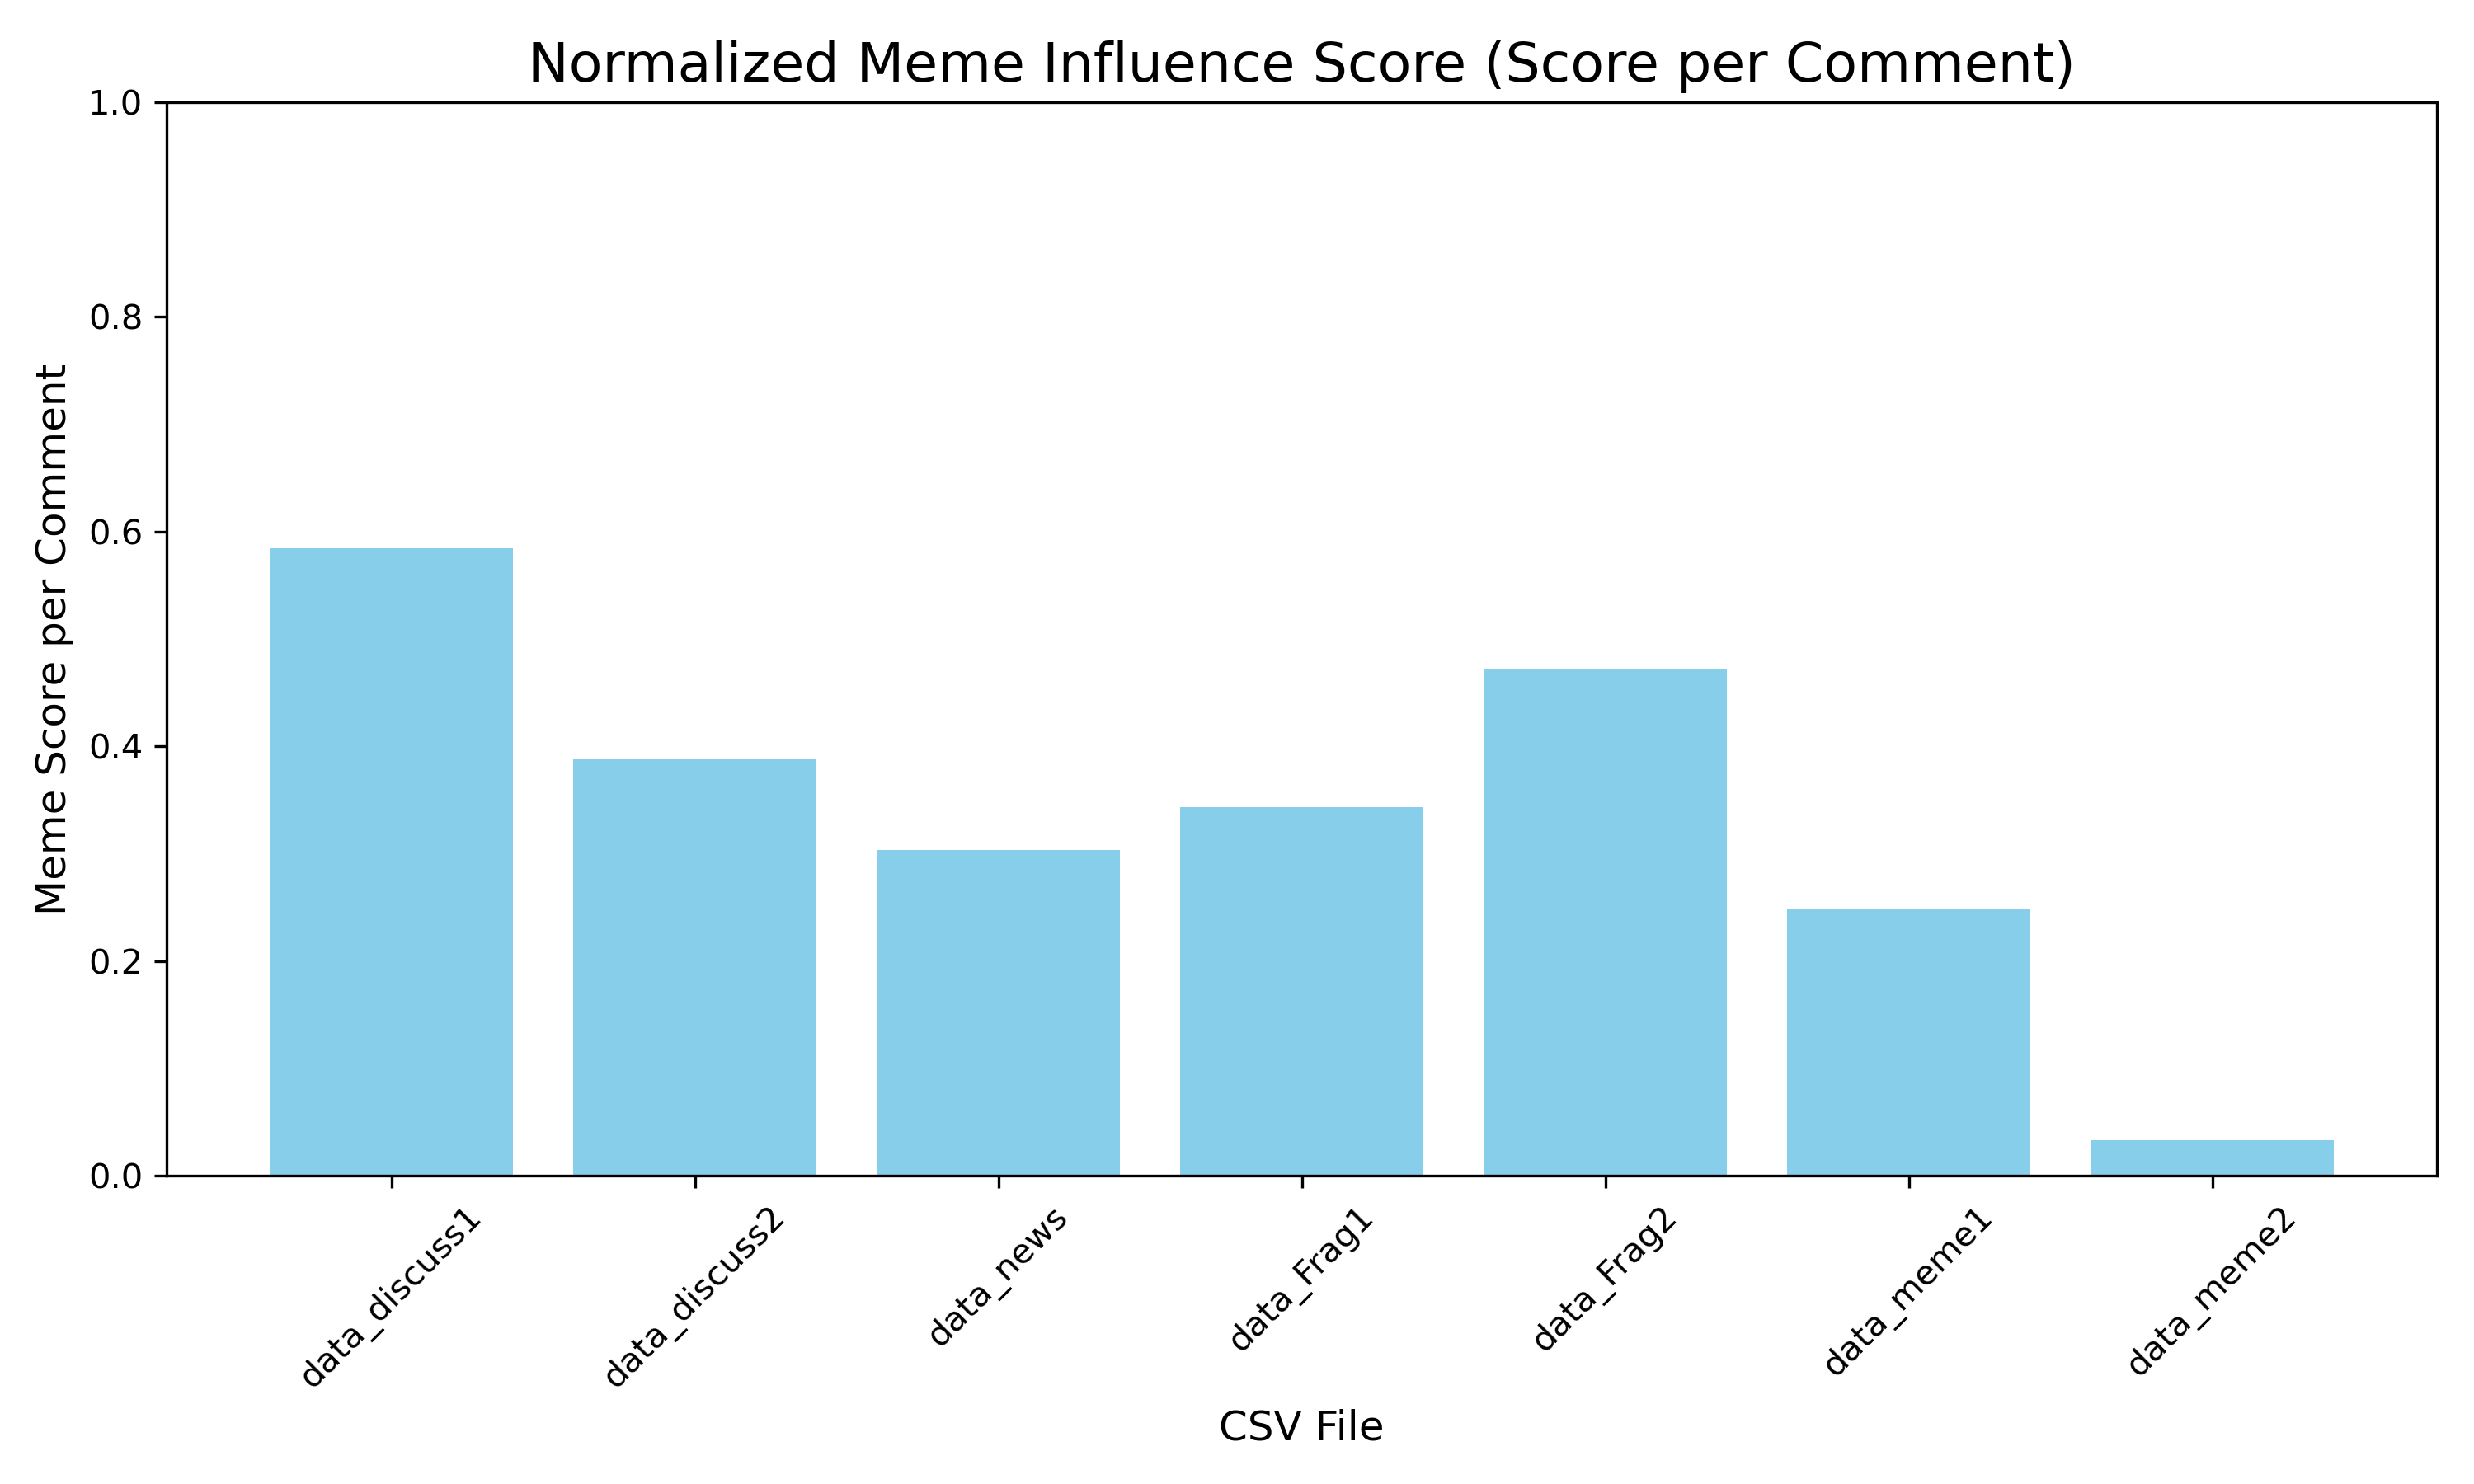
\includegraphics[width=0.8\textwidth]{img/meme_score.png}
\end{figure}
\newpage

Then, the data of the seven comment areas were evaluated through aggression evaluation, and the statistical results are as follows: it can be seen that the comment areas of the two videos directly discussing the stray cat problem and the video about the news of stray cats showed significantly stronger aggression, while the language of the two secondary creations based on the stray cat problem was significantly less aggressive than the other samples.

\begin{figure}[htbp]
    \centering
    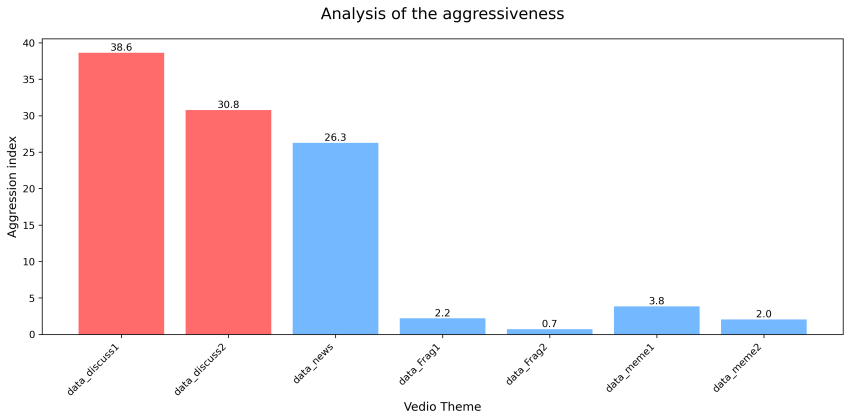
\includegraphics[width=0.8\textwidth]{img/aggressive_analysis.png}
\end{figure}
\newpage

Based on the aggressiveness assessment, the aggressiveness of comments in the comment area was evaluated, and the average level of aggression of comments on the same day was counted according to the release time, and the distribution of aggression in the comment area over time was obtained.
The statistical results are as follows
data discuss1.csv | number of comments:11608 | 2021-09-01 ~ 2025-05-14
data discuss2.csv | number of comments:304 | 2022-10-26 ~ 2024-02-22
data news.csv | number of comments:1458 | 2023-08-04 ~ 2025-05-14
data Frag1.csv | number of comments:480 | 2025-03-25 ~ 2025-05-14
data Frag2.csv | number of comments:1667 | 2025-03-19 ~ 2025-05-13
data meme1.csv | number of comments:3205 | 2025-03-23 ~ 2025-05-14
data meme2.csv | number of comments:2369 | 2025-02-06 ~ 2025-05-14

\begin{figure}[htbp]
    \centering
    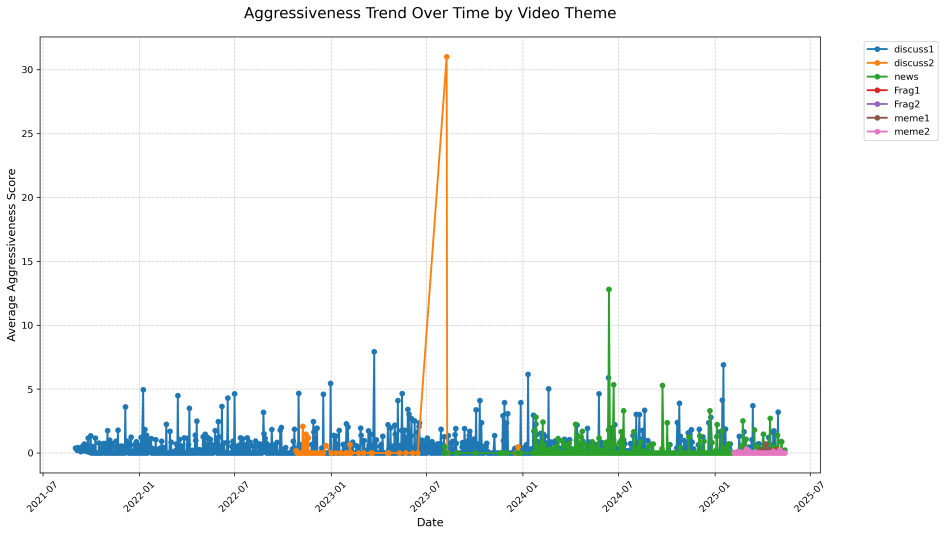
\includegraphics[width=0.8\textwidth]{img/aggressive_trend.png}
\end{figure}
\newpage

The comment area of the discussion about stray cats showed a significant high level of aggression, showing two different manifestations: one with a significantly higher level of aggression for a long time, and the other with a high peak of aggression level much greater than that in other comment areas.

News about stray cats is highly aggressive in the comment section, but this aggression gradually decreases after reaching its peak.

The comment section of other works is significantly less aggressive, and most of them do not have large fluctuations.

It can be seen that the topic relevance from the sample "discuss1" to "meme2" in the comment area shows a downward trend, which means that the discussion of the topic of stray cats in the comment area has decreased significantly with the shift of the video topic, and with the popularity of "elderly" meme, this term is no longer used when only talking about stray cats.

\begin{figure}[htbp]
    \centering
    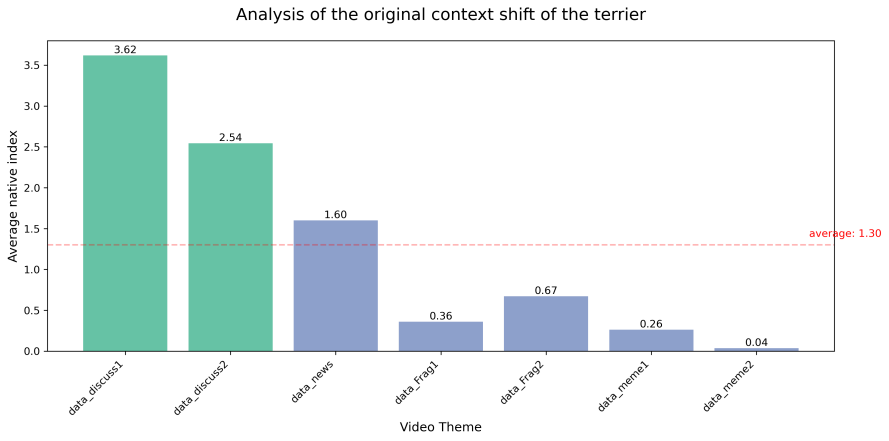
\includegraphics[width=0.8\textwidth]{img/context_shift.png}
\end{figure}
\newpage

Combined with the thematic diversity evaluation system, we extracted the hot topics discussed in the seven comment areas, and the statistical results are as follows

Subject Vocabulary for each document:

data discuss1:

Topic 1: 流浪, 一只, 喜欢, 真的, 绝育, 小区, 但是, 领养, 知道, 就是

Topic 2: 流浪, 安乐死, 问题, 绝育, 捕杀, 人士, 就是, 不是, 爱猫, 直接

Topic 3: 回复, 视频, doge, up, 这个, 老鼠, 评论, 一个, 建议, 一下

Topic 4: 生态, 家猫, 我国, 人类, 老鼠, 就是, 这个, 还是, 论文, 物种

Topic 5: 流浪, 人类, 动物, 物种, 城市, 数量, 生态, 因为, 不是, 就是

data discuss2:

Topic 1: 流浪, 哈哈哈哈, 哈哈哈, 喜欢, 微笑, 可爱, 觉得, 真的, call, 不是

Topic 2: doge, 脱单, 流浪, 回复, 吃瓜, up, 人类, 清道夫, 喜欢, 视频

Topic 3: up, 滑稽, 建议, 小黑子, 不想, 流浪, 关注, 蟑螂, 是不是, 扑杀

Topic 4: 物种, 流浪, 入侵, 危害, 放生, doge, 本土, 这么, 处理, 不能

Topic 5: 流浪, 动物, 保护, 一个, 还是, 如果, 喜欢, 不是, 应该, 领养

data news:

Topic 1: 垃圾, 这个, 射箭, 视频, up, 精英, 合肥, 不是, 如果, 邀请赛

Topic 2: 流浪, 动物, 物种, 捕杀, 保护, 亿只, 造成, 生态, 入侵, 鸟类

Topic 3: 流浪, 还是, 哈基米, 小区, 弓箭, 这种, 别人, 不是, 容易, 东西

Topic 4: 回复, 就是, 野猫, 真的, 哔哩, 流浪, 一下, 人类, 喜欢, 要是

Topic 5: 致敬, 传奇, 英雄, 支持, 复合弓, 韦鲁斯, 危险, 建议, 处理, 弹弓

data Frag1:

Topic 1: 眼睛, 老鼠, 暹罗, tv, 哈吉, 还是, 真的, 这个, 支持, 音乐

Topic 2: 我家, 星星, 这个, 知道, 一只, 豪猫, 神人, 就是, 忍住, 还是

Topic 3: 喜欢, 养猫, 这么, 这种, 不如, doge, 穿越, 看片, 东西, 起来

Topic 4: doge, 金箍, 主人, 一个, 突然, 回复, 耗子, 猫猫, 永远, 攻击

Topic 5: 哈气, 养猫, 应激, 视频, 家里, 这些, 笼子, 直接, 足球, 你们

data Frag2:

Topic 1: doge, 智商, 刺猬, 看到, 鼠饼, 一次, 狗饼, 出来, 还有, 见过

Topic 2: 看到, 就是, 直接, 过去, 马路, 知道, 体型, 经常, 比较, 所以

Topic 3: 原因, 滑稽, 就是, 撞死, 红绿灯, 我家, 小猫, 见到, 比较, 缝缝补补

Topic 4: 因为, 聪明, 还是, doge, 流浪狗, 一般, 主要, 不是, 而且, 金箍

Topic 5: 看见, 哈气, 哈基米, 狗子, 看到, 高速, 时候, 一个, 不少, 压死

data meme1:

Topic 1: 不是, 野猫, 一只, 流浪, 经典, 还是, 但是, 这种, 如果, 这么

Topic 2: 啊啊啊, 足球, 表情, 星星, 一个, 已经, 我力, 骇死, 宝宝, 汤圆

Topic 3: doge, 这个, 这种, 金箍, 视频, 哈基人, 手套, 飞舞, 遇到, 那个

Topic 4: 直接, 哈基米, 我家, 这样, 哈基, 然后, 基米, 神人, 过去, 忍住

Topic 5: 哈气, 可爱, 知道, 相思, 就是, 哈基米, 圆头, 大哭, 感觉, 这猫

data meme2:

Topic 1: 原版, 猎奇, 这个, 感觉, 武器, 眼睛, 吓人, 可爱, 哈基米, 超越

Topic 2: 骇死, 我力, doge, 补档, 啊呀, 缓存, 视频, 还有, 这么, byd

Topic 3: 视频, 出来, 恐怖, 真的, 一个, 支持, 这个, 孩子, 东西, 一只

Topic 4: 哈气, 回复, 表情, 这个, mygo, 哔哩, 视频, 不是, 因为, 喜欢

Topic 5: 看过, 微笑, official, 还原, 知道, tv, 程度, 不要, 一下, 骇人

\begin{figure}[htbp]
    \centering
    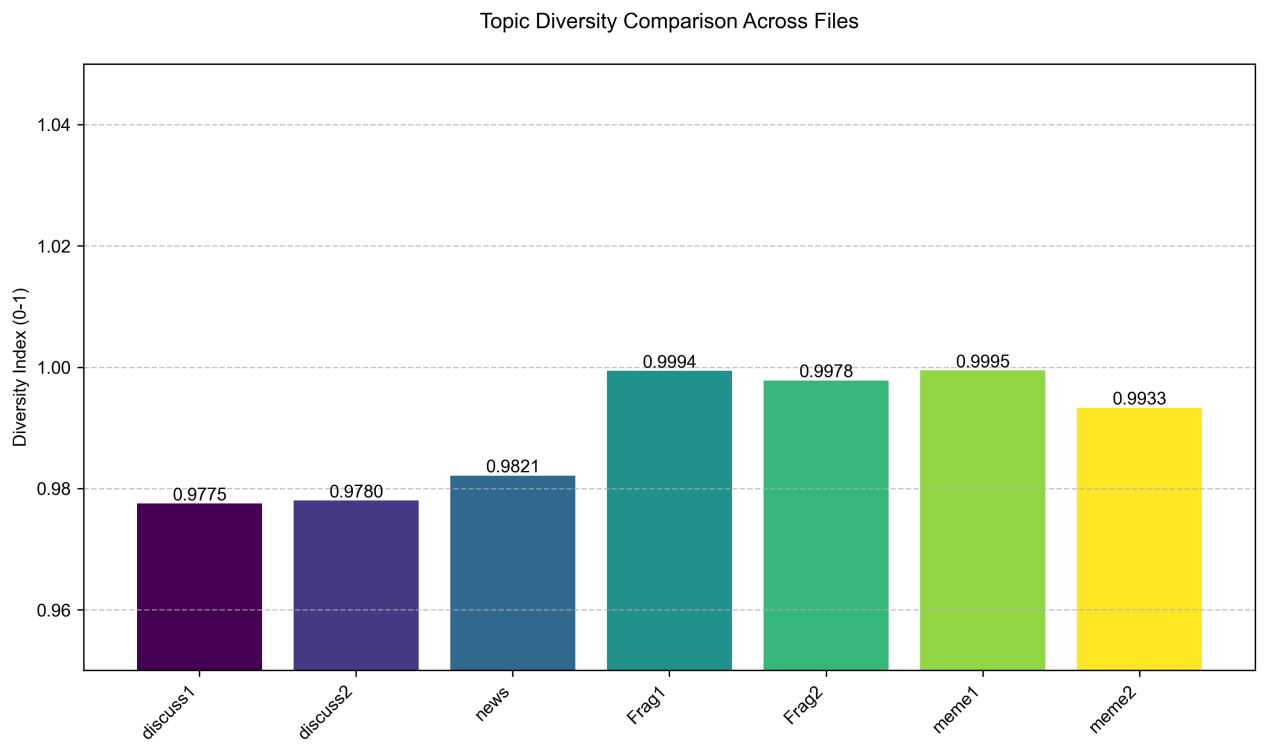
\includegraphics[width=0.8\textwidth]{img/topic_diversity.png}
\end{figure}
\newpage

The topic of cats is decreasing, more meme cultures such as "Hakimi" and "Hacking me" appear in the comment section, and the discussion videos of stray cats with high scores on aggression evaluation score are significantly lower in terms of topic diversity.

\subsection{Result analysis}

With the popularity of memes, its context gradually detached from the original problem and evolved into an independent Internet cultural phenomenon.

The aggressiveness in the comment area is highly correlated with the nature of the topic, and serious social issues are easy to trigger highly aggressive discussions, while with the popularity of memes, the topic changes to more entertaining non-serious topics, which shows a dissipating effect on the violence of language.

The analysis of the theme reveals the trend of online language from the discussion of practical problems to the culture of pluralism and memes.

This experiment provides quantitative support for understanding the influence of abstract culture on the characteristics of online language, and reveals the dynamic change characteristics of aggressive language in online discussion.

\section{Discussion}

This experiment conducted a preliminary exploration of the relationship between abstract culture and cyberbullying by surveying various aspects of internet users' behavior in online spaces.

Most survey participants had at least a basic or relatively good understanding of abstract culture, indicating the prevalence of abstract culture is widespread among young people. However, we acknowledge that the survey results may suffer from significant survivorship bias, as respondents were more likely to be individuals deeply embedded in online communities with ample leisure time for internet entertainment. Thus, while the survey does not prove the universality of abstract culture across all demographics, it does demonstrate the widespread use of abstract language in transmitting information across the internet.A larger survey may be able to better characterize the relationship between abstract culture and a larger group of people

We observed that most participants had a good grasp of abstract culture, yet the vast majority believed they had neither experienced nor participated in cyberbullying. One possible explanation is that many netizens may not recognize subtle, abstract forms of violent insinuations directed at them. Another possibility is that most cyberbullying incidents are short-lived, eventually evolving into broader, longer-lasting meme behaviors over time.

While the survey focused on the behaviors of online communities, our analysis of comment data prioritized the evolution of specific abstract phenomena. Through manual examination of comments under videos related to the Mao-Die meme, we found that after 2023, the abstract and metaphorical nature of comments significantly increased—a trend linked to the rise of abstract culture. Abstract expression transcended its original boundaries of pure entertainment and, in videos resembling news content, lost some of its playful tone, instead being imbued with stronger satirical, political, and reflective meanings by netizens.

A detailed analysis of sample files data discuss1 and data meme1 reveals that comments in 2023 markedly differed in style from those in 2021. Commenters increasingly favored abstract, humorous language to critique serious social issues. By 2025, the popularity of derivative entertainment videos on this topic even surpassed that of 2021. The focus of discussions shifted from real-world issues (such as stray animals) to the internet-famous cat itself, becoming more lighthearted and less satirical or metaphorical. Only a minority remained aware of the original context, while the majority engaged purely for entertainment. This aligns with our hypothesis that the violent potential of abstract language diminishes as abstract culture becomes more mainstream.Although our evaluation scheme for the comment area data provides an explanation for the characteristics of online language, such an evaluation is not complete, especially the concealment and diversity of online language violence, which puts forward the requirement for a more detailed and comprehensive evaluation system

\section{References}
%参考文献部分
%jieba库
%LDA
%代码开源位置























%**************问卷调查暂存在此
\section{Old version}
\subsection{Questionnaire Survey}

Objective: To investigate the understanding of meme culture among different age groups, genders, and education levels, as well as their perception of the relationship between meme culture and cyberbullying.

Survey Results (intact Analysis):

Figure 2 shows the age distribution of the respondents, and it can be seen that the participants are mainly concentrated in the age group of 15-25 years old, that is, post-zeros, who are also the main participants in online activities.

\begin{figure}[htbp]
    \centering
    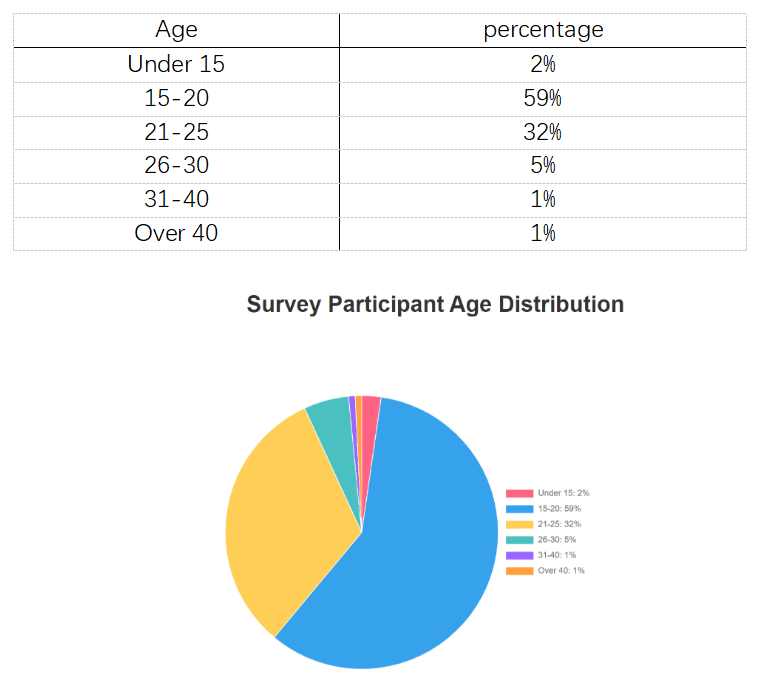
\includegraphics[width=0.8\textwidth]{img/age_distribution.png}
    \caption{Age Distribution of Participants}
    \label{fig:age_distribution}
\end{figure}
\newpage

Figure 3 shows the age distribution of participants using the Internet for the first time and it also shows the age of the participants. It can be seen that three-quarters of the participants in the primary and secondary school stage of the first contact network, and three-quarters of the participants have four years or more of the Internet experience, which proves that most of the respondents in this questionnaire survey have rich network experience.

\begin{figure}[htbp]
    \centering
    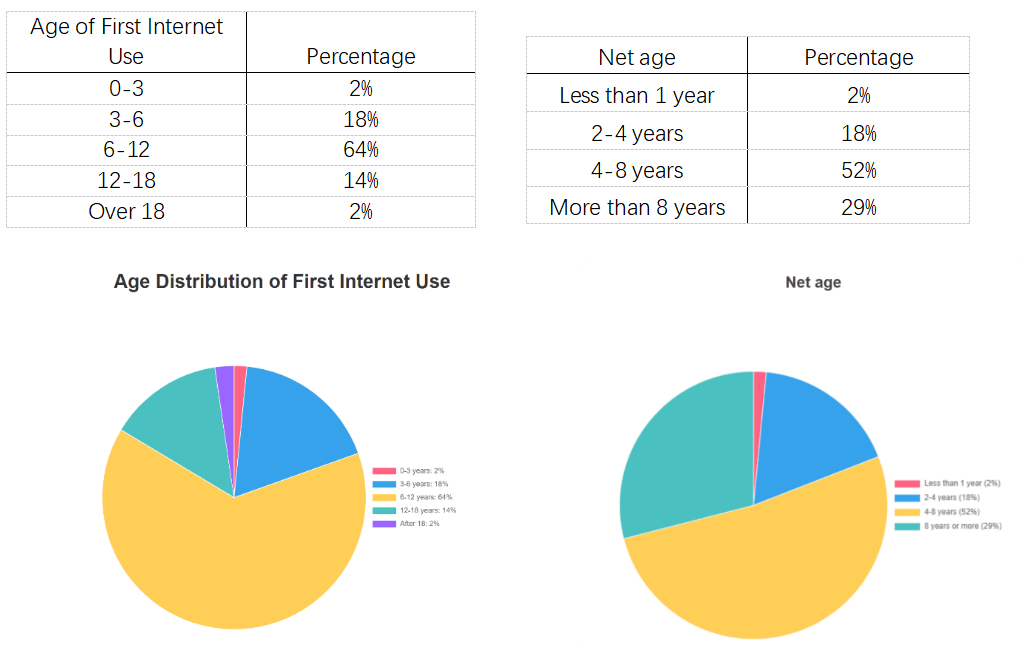
\includegraphics[width=0.8\textwidth]{img/first_use_age_distribution.png}
    \caption{Age Distribution of First Internet Use}
    \label{fig:first_use_age_distribution}
\end{figure}
\newpage

Figure 4 shows the correct response rate of the abstract meme test, and the correct distribution of the participants is relatively normal, with most people having a basic or somewhat understanding of abstract culture (between 30\% and 80\% correct rate), and only a small number of people have little or very good understanding of abstract culture (less than 30\% or more than 80\% correct rate). It can be concluded that abstract culture has a good popularity.

\begin{figure}[htbp]
    \centering
    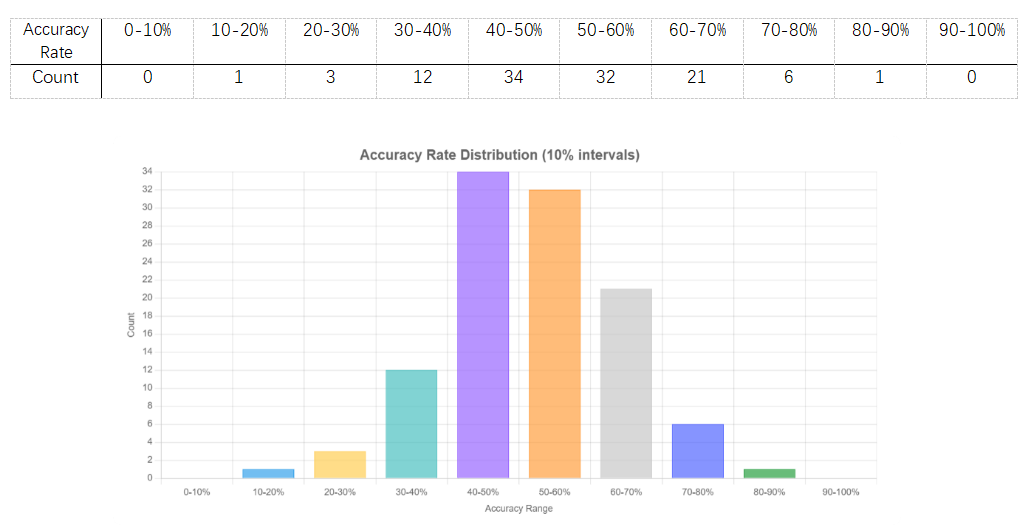
\includegraphics[width=0.8\textwidth]{img/abstract_test_accuracy.png}
    \caption{Accuracy Rate Distribution(10\% intervals)}
    \label{fig:abstract_test_accuracy}
\end{figure}
\newpage

Figure 5 shows the relationship between respondents' accuracy and Internet age, while Figure 6 shows the relationship between respondents' accuracy and their age of first Internet use. After ignoring the data with too few samples (the sample size is less than five), it can be seen that the age of the Internet and the age of using the Internet for the first time have little impact on the accuracy rate, which proves that the popularity of abstract culture is universal among young people, and they can have a certain understanding of abstract culture regardless of the length of time they have been exposed to the Internet.

\begin{figure}[htbp]
    \centering
    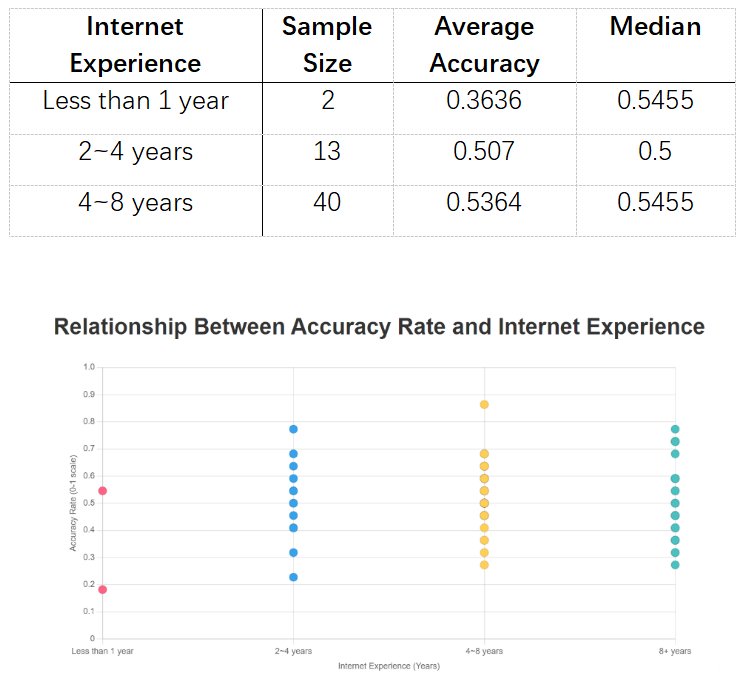
\includegraphics[width=0.8\textwidth]{img/accuracy_vs_net_age.png}
    \caption{Relationship between Accuracy Rate Internet Experience}
    \label{fig:accuracy_vs_net_age}
\end{figure}
\newpage

\begin{figure}[htbp]
    \centering
    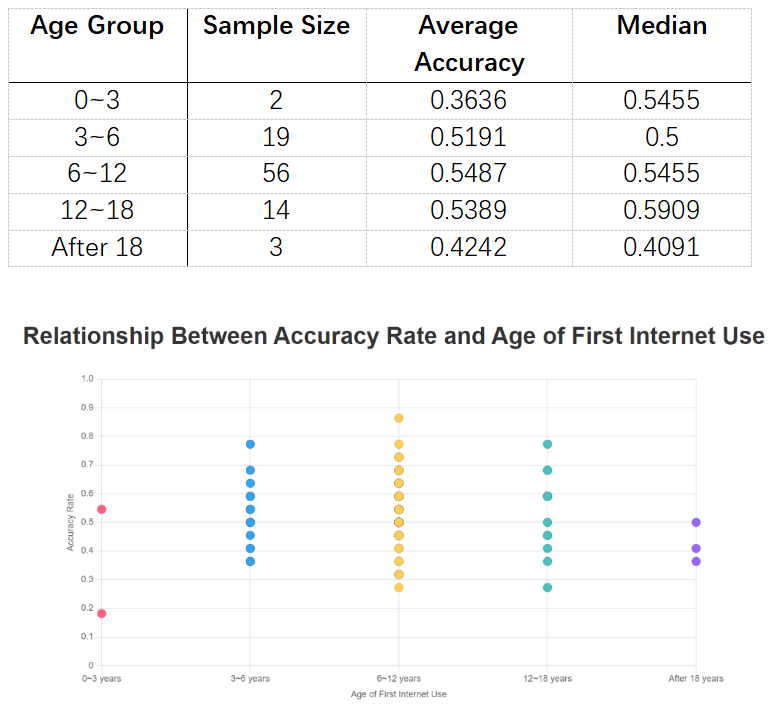
\includegraphics[width=0.8\textwidth]{img/accuracy_vs_first_use_age.png}
    \caption{Relationship between Accuracy Rate and Age of First Internet Use}
    \label{fig:accuracy_vs_first_use_age}
\end{figure}
\newpage

Next, we analyze the connection between abstract culture and online violence. As can be seen from Figure 7, more than 40\% of people are sure that abstract culture can lead to online violence, only a small number of people do not believe that abstract culture can lead to online violence, and many people are neutral.

\begin{figure}[htbp]
    \centering
    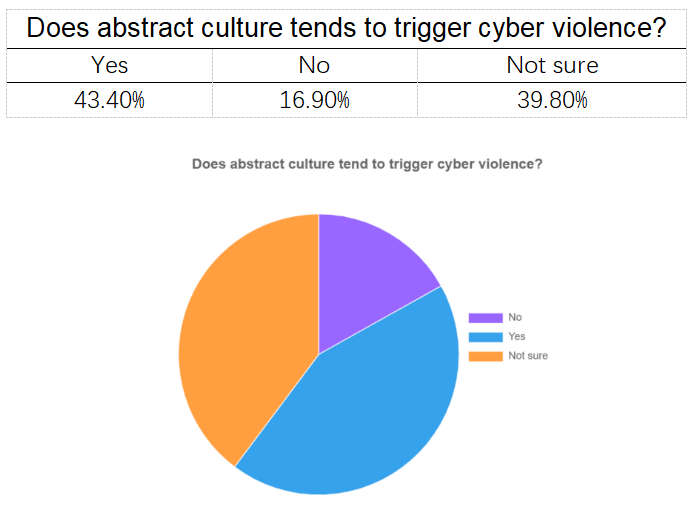
\includegraphics[width=0.8\textwidth]{img/abstract_vs_net_violence.png}
    \caption{Does Abstract Culture Tends to Trigger Cyber Violence?}
    \label{fig:abstract_vs_net_violence}
\end{figure}
\newpage

After that, we made a scenario to construct the online conversation in a way that simulates abstract culture. Here's how the scenario was designed:

Scenario Description (The Chinese text needs to be retained due to the context.)

Scenario 1: Discussion on the gaming forum

A:你这套出装根本不行,实战里就是送人头。

B:你玩过几场啊就在这指点江山?

A:急了?

Scenario 2: Comment section of prank videos

A:第二桶泡面难吃,那为什么不先吃第二桶再吃第一桶呢?

B:不对,我觉得这样第一桶就变成第二桶了。

C:乐子,没看见人家在玩抽象?

Scenario 3: Debate Among Fans of Social Media Stars

A:你家哥哥这演技也能叫好?粉丝滤镜真厚。

B:你行你上啊,键盘侠就会bb。

A:这就急了?(小丑emoji)

Scenario 4: Bickering on the forum

A:废物也就只能躲在屏幕后吠了,现实里敢吭一声?

B:你妈没教你怎么说话是吧?

A:急得开始咬人了?建议回炉重造哦。(微笑emoji)

Scenarios 1 and 2 reflect the conversations in the comment areas of game forums and some live videos in daily life, with a large number of participants and a wide range of popularity. Scenarios 3 and 4 reflect conversations such as fan arguments and scolding each other, with a focus on a specific group of people and a limited range of popularity.

As shown in Table 8 and Figure 8, more than 60\% of people in scenarios 1 and 2 believe that there is no violence or only mild violence, and less than 1 in 10 people believe that it is severe violence, which is significantly less severe. Scenarios 3 and 4 suggest that the number of people with moderate and severe violence has increased significantly, indicating that the level of violence is more severe.

From this situational survey, we can conclude that the degree of violence of abstract culture decreases when the popularity increases. This echoes the birth and development of abstract culture, which is often born in the communication of small groups with a strong offensive purpose, and after widespread dissemination, people pay more attention to its entertainment and weaken the aggressiveness.

\begin{figure}[htbp]
    \centering
    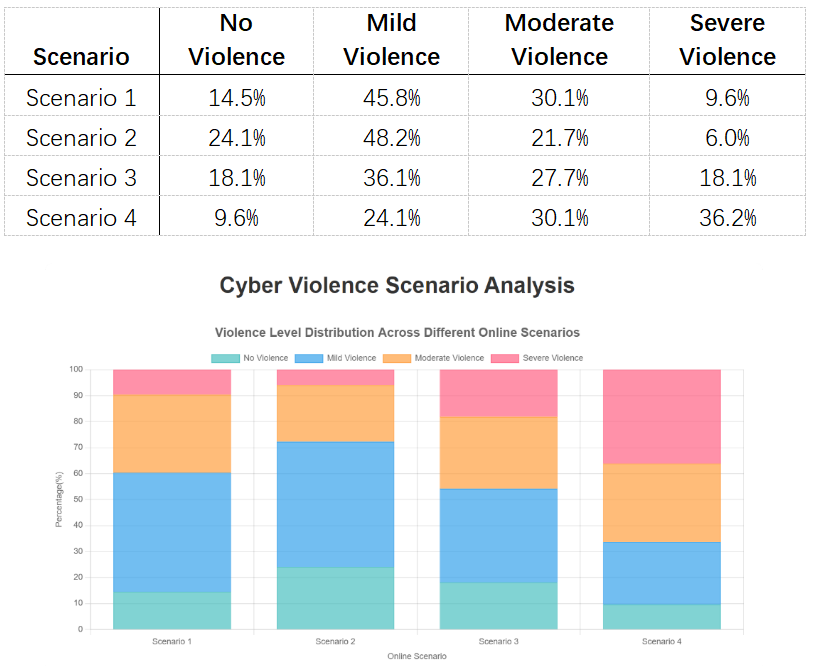
\includegraphics[width=0.8\textwidth]{img/scenario_vs_net_violence.png}
    \caption{Cyber Violence Scenario Analysis}
    \label{fig:scenario_vs_net_violence}
\end{figure}
\newpage

In summary, this survey shows that abstract culture has a wide range of awareness among young netizens aged 15-25, and there is no significant correlation between the level of awareness and the age of the Internet. The majority of respondents believe that abstract culture is prone to online violence, especially in certain small circles. The study found that with the expansion of the spread of abstract culture, its violent tendency will be relatively weakened, which indicates that there is an inverse relationship between epidemic and violence.

\end{document}
